\section{Proposed Metric}
Since BLEU did not reflect well the semantic accuracy of migrated code, there is a need for an alternative metric that can fit better with the task. The nature of the task is to compare source code in term of semantics. 
\subsection{Exploratory Study}
We did an exploratory study to verify the 3 metrics SED, TREED, and GVED. Our study reveal their correlation with the ground truth Semantic score in order to find out the best metric to evaluate SMT-based Code Migration system. Table \ref{table:correlation} summarizes our results for the two models mppSMT and lpSMT. We will explain each metric \rq s correlation in details in the following subsections. 

\begin{table}
\caption{Correlation Coefficients with Semantic score}
\begin{tabular}{|c|c|c|c|c|}
\hline
& BLEU & SED & TED & GVED\\
\hline
mppSMT & 0.524 & 0.549 & 0.684 & 0.862 \\
lpSMT & 0.621 & 0.635 & 0.774 & 0.836 \\
\hline
\end{tabular}
\label{table:correlation}
\end{table}


\subsubsection{\textbf{SED vs Semantic}}
SED is similar to BLEU in the way that both of them compare source code as token sequences at lexical level. That is confirmed and reflected in our empirical result. Indeed, the two metrics have similar correlations with Semantic score (table \ref{table:correlation}. The correlation coefficient increases from 0.524 to 0.549 (mppSMT), and 0.67 to 0.675 (lpSMT). Nevertheless, the improvements are too trivial that can be ignored. SED suffers the same drawback as BLEU: it does not take into consideration the structures of source code, and it only compares source code in term of lexemes. 
%that SED would deduce more penalty if the translated method has incorrect order of lexeme tokens. 
So, it is not worth to use SED instead of BLEU since it still has the same problems as BLEU while its advantage is insignificant. 

%\begin{figure}
%\caption{SED vs Semantic (lpSMT)}
%\centering
%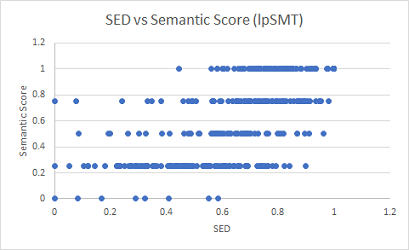
\includegraphics{img/sedvssem_lpSMT.png}
%\label{fig:SedSemlpSMT}
%\end{figure}
%
%\begin{figure}
%\caption{SED vs Semantic (mppSMT)}
%\centering
%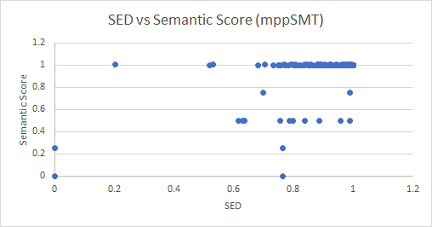
\includegraphics{img/sedvssem_mppSMT.png}
%\label{fig:SedSemMppSMT}
%\end{figure}

\subsubsection{\textbf{TREED vs Semantic}}
TREED compares source code at higher level of representation (Syntax Tree). Syntax of source code is the pre-requisite before mentioning about its semantics or functionality. Comparing methods in term of syntax is likely to reflect semantic accuracy better than comparing at lexical level. This argument is proved by our empirical results: 

%Technically, a translated method cannot be said to perform any functionality if it cannot be compiled. However, in the Code Migration problem, a translated method which has wrong syntax can still be useful for developers. 

Figure \ref{fig:TREEDmppSMT} shows the scatter plots between 2 metrics: TREED and Semantic. In general, the figure has similar trend as BLEU's one: The data points are too scattered to show a noticeable correlation and there are several outliers. For a fixed value of Semantic score, TREED score can still vary in a large range. However, comparing to BLEU, the variety is much smaller. For example, a [pair of method that has Semantic score of 0.5 can possibly have TREED scores in range of 0.7 to 1 while such range is 0.5 to 1 for BLEU. TREED shows some noticeable improvements on the correlation with Semantic score on mppSMT model (0.524 to 0.684), and on lpSMT model (0.621 to 0.774). 

%\emph{Observation 1:} For a fixed value of Semantic score, there can be many associated TREED values. Specifically, in the model lpSMT, with a Semantic Score of 1, the TREED scores can be varied greatly between 0-1, which was reflected on the top horizontal line of dots in figure \ref{fig:TREEDlpSMT}. Similarly, in the figure \ref{fig:TREEDmppSMT}, with a Semantic Score of 1, the TREED scores are in the range of 0.7 to 1. 
%
%\emph{Observation 2:} For a fixed value of TREED, there can be many associated Semantic scores. For example, the figure \ref{fig:TREEDlpSMT} shows that for a high TREED score, for example 0.8, can have Semantic Score from 0.25 to 1. This can be observed by the vertical line of dots in the figure. 



% Comparing figure \ref{fig:BleuSemMppSMT} and figure \ref{fig:TREEDmppSMT}, it can be realized that on the model mppSMT, those horizontal lines of dots in figure \ref{fig:BleuSemMppSMT} became shorter in figure \ref{fig:TREEDmppSMT}. It means the variation of TREED score for certain Semantic score is lower. Data points in the figure can also be approximately fitted with a regression line even though there still are some outliers. 

%From observation 1, it can be implied that a translated method can have low TREED score, but high Semantic score. On the other hand, from observation 2, a translated method can have high TREED score, but low Semantic score. The two implications above shows that an improvement in TREED is not sufficient nor necessary to improve translation migration quality. However, from observation 3, there is hint of positive improvement that using TREED would reflect Semantic score better than BLEU. 

In general, TREED still suffers the same issues with BLEU even though the reasons are different for the two metrics, and TREED was effected in lesser degree. A translated method can be perfectly compilable, but still fails to capture functionality of the reference one (high TREED score, low Semantic score). On the other hand, there exists the situation of low TREED score, but high Semantic score. For example, translated method can have incorrect position for a semicolon which makes it impossible to compile. Beside that only mistake, if it can reflect the functionality of the reference code, a human subject could still it give a high Semantic score. However, due to the increase of coefficient, there is hint of potential that using TREED would reflect Semantic score better than BLEU. For certain circumstance, TREED could be used to evaluate SMT-based Migration system that focuses on translating correct syntax code. 

%\begin{figure}
%\caption{TREED vs Semantic (lpSMT)}
%\centering
%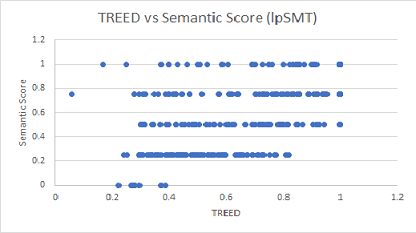
\includegraphics{img/treed_lpSMT.png}
%\label{fig:TREEDlpSMT}
%\end{figure}
%
\begin{figure}
\caption{TREED vs Semantic (mppSMT)}
\centering
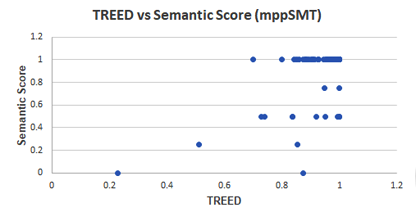
\includegraphics{img/treed_mppSMT.png}
\label{fig:TREEDmppSMT}
\end{figure}

\subsubsection{\textbf{GVED vs Semantic}}
Comparing source code in term of structure (specifically PDGs in our study) to estimate semantic similarity is the 
highest level of comparison. PDGs capture all data and control dependence of program elements, and those dependencies are the keys to reflect functionality of source code. Therefore, GVED is expected to have the best correlation with Semantic score. Our results cement this argument. 

Figure \ref{fig:GVEDmppSMT} shows the scatter plots between 2 metrics: GVED and Semantic score when GVED is applicable. There are 240 of such points for the model mppSMT in the total of 375 pairs of methods, and respectively 75 points for lpSMT. The correlation coefficient between GVED and Semantic score for the model mppSMT is 0.893 and for the model lpSMT is 0.980. They show significant improvements on both models comparing to any of the other 3 metrics. All other 3 metrics have correlation coefficients with Semantic Score less than 0.7 while GVED achieves remarkable correlation coefficients of nearly 1.0. GVED's promising result makes it an obvious choice to evaluate SMT-based Code Migration systems. However, such systems always have the problem that the translated methods have too many errors that cannot be built into PDG, or even be compiled. That explains the situation
in which the number of data points available for model lpSMT is too small to draw conclusion about the correlation with high confidence. 

Therefore, even though GVED is a reliable metrics, it is not always applicable. To cope with GVED limitation while still utilize its strong indication of semantic accuracy, we propose our novel metric: {\model}. 

%\begin{figure}
%\caption{GVED vs Semantic (lpSMT)}
%\centering
%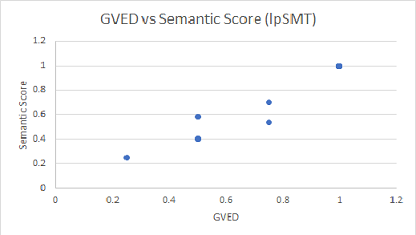
\includegraphics{img/gved_lpSMT.png}
%\label{fig:GVEDlpSMT}
%\end{figure}
%
\begin{figure}
\caption{GVED vs Semantic (mppSMT)}
\centering
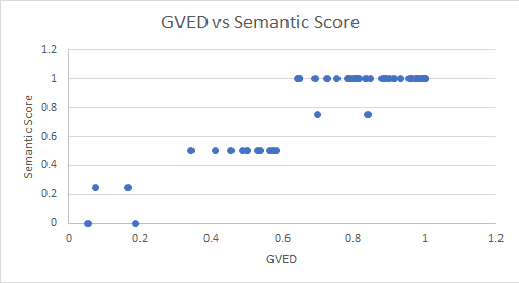
\includegraphics{img/gved_mppSMT.png}
\label{fig:GVEDmppSMT}
\end{figure}
\subsection{Design}
In this subsection, we propose {\model}, a novel automated metric to evaluate SMT-based code migration tools that is suitable for source code, is language independence, can reflect well the semantic accuracy of translated results, and inexpensive to compute. {\model} is then validated on practical SMT-based code migration models to show its potential and effectiveness. 

\emph{Insight 1 :} In computer network, a best effort delivery describes a network service that does not guarantee the quality of delivery. Nevertheless, the service will make their "best effort" to try to deliver the packet with its available resources. Under some circumstances, the packet may be loss or delayed. Similarly, in the domain of SMT-based Code Migration problem, a translated method cannot be guaranteed to be compilable or be built into PDG. Regardless, we would try our best effort to measure its semantic similarity with respect to the reference method as accurate as possible. \\
\emph{Insight 2 :}
According to Table \ref{tab:summary} in section 5, there is a trend of increasing correlation coefficient with Semantic score when more complex levels of source code are used. Specifically, GVED has the highest correlation, and it follows by TREED, SED, BLEU respectively. Therefore, those metrics should have priority order when be used in evaluating translation results.  

From the two insights, we design {\model} as a best-effort multi-layered metric. {\model} is a combination metric that takes into consideration metrics at the lexical, syntactical, and semantic levels of source code while aims to measure the semantic accuracy of translated code in a reliable manner. If the translated code can be built into PDG, we calculate {\model} in term of graph vector edit distance (GVED). If the translated code cannot be built into PDG, but is compilable, {\model} is calculated as syntax tree edit distance (TREED). Lastly, if the translated code is not compilable, we use string edit distance (SED) to compute {\model}.

The formula of {\model} is presented in Algorithm \ref{ruby}. GVED, TREED, and SED were defined in section 4.3. $r$ is the reference code, $t$ is the translated code; in turn $r,t$ are tokenized into sequences to use in SED, are parsed into ASTs to use in TREED, and are built into PDGs to use in GVED.  
\makeatletter
\def\BState{\State\hskip-\ALG@thistlm}
\makeatother
\begin{algorithm}
\caption{Calculate {\model}}\label{ruby}
\begin{algorithmic}[1]
\If { $\mbox{GVED}\left(r,t\right) $ is applicable }
\State $\mbox{RUBY}\left(r,t\right) = \mbox{GVED}\left(r,t\right) $
\ElsIf { $\mbox{TREED}\left(r,t\right) $ is applicable }
\State $\mbox{RUBY}\left(r,t\right) = \mbox{TREED}\left(r,t\right) $
\Else 
\State $\mbox{RUBY}\left(r,t\right) = \mbox{SED}\left(r,t\right) $
\EndIf
\end{algorithmic}
\end{algorithm}

\subsection{Proposal result}

To evaluate RUBY, we conducted the same experiment with other four
metrics to show the correlation of RUBY with semantic scores on two
model mppSMT and lpSMT. RUBY's efficiency was tested on a large number
of methods translated by those models.

\begin{figure}[t]
\caption{RUBY vs Semantic (lpSMT)}
\centering
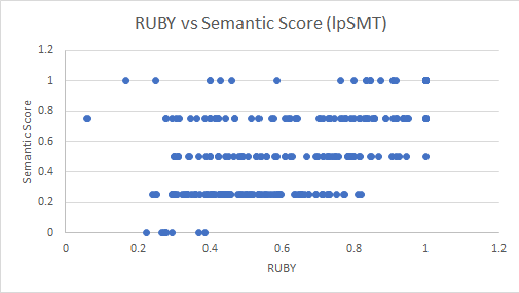
\includegraphics{img/rubyvssem_lpSMT.png}
\label{fig:RubySemlpSMT}
\end{figure}

\begin{figure}[t]
\caption{RUBY vs Semantic (mppSMT)}
\centering
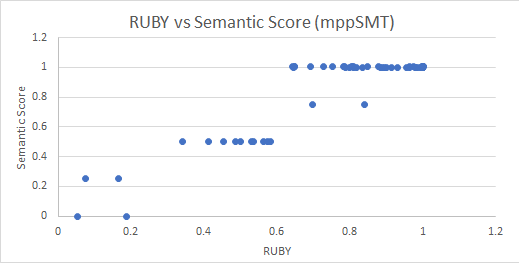
\includegraphics{img/rubyvssem_mppSMT.png}
\label{fig:RubySemMppSMT}
\end{figure}

Figures~\ref{fig:RubySemlpSMT} and~\ref{fig:RubySemMppSMT} show the
scatter plots between RUBY and Semantic scores on two models mppSMT
and lpSMT, respectively. As can be seen from the scatter plot for
lpSMT (Figure~\ref{fig:RubySemlpSMT}), there is a moderately strong,
positive, linear association between the two variables with a few
outliers.  Beside, the scatter plot for mppSMT
(Figure~\ref{fig:RubySemMppSMT}) shows a strong, positive, linear
association between RUBY and Semantic score. There are no outliers in
the data. This is the indication that the result is consistent.

In general, RUBY has high correlation with Semantic scores. As our
experiment result, the correlation coefficient between RUBY and
semantic score for model mppSMT is \textbf{0.862} and for the model
lpMSMP is \textbf{0.836}. In statistics, these values indicate a
strong uphill linear relationship between two quantitative
metrics. That means one metric could be predicted by the other with
high confidence. For example, an increase of 0.5, {\model} score can
be interpreted as an increase of 0.4 in term of Semantic score. Based
on that information, developers can tune the system in an incremental
manner.


%Specifically, a correlation of +0.8 implies that when 	

Although RUBY has a strong correlation coefficient, it is still lower
than GVED scores shown in Section~\ref{sec:alternatives} due to the
fact that only a subset of the dataset is applicable. While GVED is
only computed with the migrated code with sufficient semantic
information, RUBY does not depend on the code, even we can not parse
PDGs and ASTs. This implies that there exist a RUBY score for any
given code. On the other hand, in comparison with TREED, SED
and BLEU, RUBY always outperforms the other three metrics.
	    
  			


\begin{figure}
\caption{RUBY vs Semantic (lpSMT)}
\centering
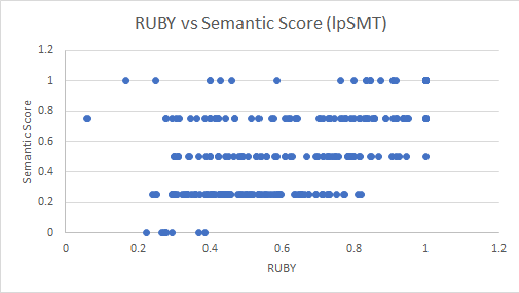
\includegraphics{img/rubyvssem_lpSMT.png}
\label{fig:RubySemlpSMT}
\end{figure}

\begin{figure}
\caption{RUBY vs Semantic (mppSMT)}
\centering
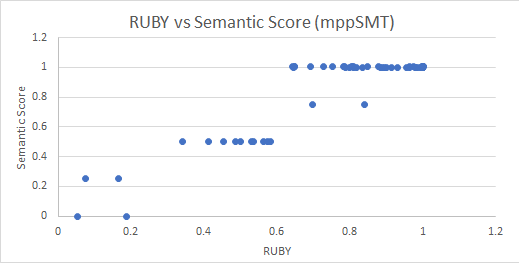
\includegraphics{img/rubyvssem_mppSMT.png}
\label{fig:RubySemMppSMT}
\end{figure}

%BLEU has always been doing this and that....

%Researchers usually claim that an improvement in BLEU also meant an
%improvement in translation quality. So 

%BLEU has been used for not only evaluating the result but also tuning
%and developing SMT-based migration system.
%%From the results in section 5, BLEU did not reflect the semantic accuracy of source code. --> We need a better metrics to replace BLEU
%However, from the results in section 5, it can be concluded that BLEU
%did not reflect well the semantic accuracy of migrated source code
%since it has weak relation with human judgments. Therefore, we need a
%better metric in order to fit better with programming languages and
%code migration systems.
%%
%%Needed metric should be 
%%Reflect semantical meaning of sources code.
%%Automated
%%Low computation's cost
%%Independent of programming language
%%Independent of MT model's type
%Such a metric should have the following requirements:
%
%
%\emph{1}. The metric is more suitable for source code than BLEU. It
%can reflect the semantics of source code and the semantic accuracy of
%translation result. To fulfill that, the metric must have high
%correlation with human evaluation for the translation result.
%
%
%\emph{2}. The metric can be computed automatically and inexpensively in
%order to support the evaluation of migration results in the
%incremental development of SMT-based code migration systems. For
%example, the metric can be calculated quickly after each iteration of
%development so a system can be evaluated and tuned in a timely~manner.
%
%\emph{3}. The metric is independent of the programming languages and
%of the SMT models. A good and reliable metric must have consistent
%results for any languages and models so it can be applied universally
%to any SMT-based code migration systems.
%
%%What is Ruby and why Ruby is good.
%Considering all above requirements, we introduce {\model}, a novel automated metric that can reflect semantic accuracy of translated code. {\model} is also independent of programming languages and machine translation models used in migration system. {\model} measures the semantic accuracy of the resulting code with respect to reference code by comparing their Program Dependence Graph (PDG). PDG captures both the data and control dependencies among program entities. Because those dependencies play an important role in a program, we expect PDG can represent well the semantics of source code. Usually, comparing graph is expensive, but our approach makes it affordable. We estimate the graph edit distance by vectorizing the graph and calculating the vectors edit distance. Because of that, we can save the computational cost and make our approach scalable. Basically, every programming language code can be built into PDG. Hence, our metric can be used for Code Migration systems that migrate different programming languages. Lastly, the way {\model} is measured makes it independent of machine translation models. That means Code Migration systems that deployed different SMT models can still use our metric. Next, we go into details how to formalize the calculation of {\model}
%
%%To reduce the high computational cost, we vectorize the PDGs and calculate the vector difference to estimate the graph difference. This way, we would make sure that our model is practical and applicable in large scaled systems. 
%
%When applying MT on source code, there always exists the problem that the translated code is broken in term of syntax. Thus, it is impossible to build PDG or even compile those code. To cope with the problem, our model is designed as best-effort, layered metric  : If the translated code can be built into PDG, we calculate {\model} in term of graph edit distance. If the translated code cannot be built into PDG but is compilable, we calculate {\model} in term of syntax tree edit distance. If the translated code is not compilable, we calculate {\model} in term of string edit distance. We then represent about the 3 metrics graph/tree/string edit distances as follows:



